\documentclass{article}
\usepackage{graphicx}
\usepackage[margin=1.5cm]{geometry}
\usepackage{amsmath}

\begin{document}
\twocolumn

\title{Friday Warm Up: Unit 5: Momentum I}
\author{Prof. Jordan C. Hanson}

\maketitle

\section{Memory Bank}

\begin{itemize}
\item $\vec{p} = m\vec{v}$ ... Definition of momentum.
\item $\vec{p}_{\rm total} = \vec{p}_1 + \vec{p}_2$ ... Total momentum.
\item $\vec{p}_{\rm total,i} = \vec{p}_{\rm total,f}$ ... Momentum is conserved.
\item $m_p = 1.67 \times 10^{-27}$ kg ... Mass of protons.
\end{itemize}

\section{Momentum}

\begin{enumerate}
\item An object that has a small mass and an object that has a large mass have the same momentum. Which object has the largest kinetic energy?
\begin{itemize}
\item A: The one with small mass
\item B: The one with large mass
\end{itemize}
\item Two objects of equal mass are moving with equal and opposite velocities when they collide. Can all the kinetic energy be lost in the collision? 
\begin{itemize}
\item A: Yes
\item B: No
\end{itemize}
\item Suppose two loaded train cars are moving toward one another, and they couple together.  The first has a mass of $1.50\times 10^5$ kg and a velocity of $0.30\hat{i}$ m s$^{-1}$, and the second has a mass of $1.10\times 10^5$ kg and a velocity of $−0.12\hat{i}$ m s$^{-1}$. What is their final velocity? \\ \vspace{3cm}
\item A proton collides with a neutron (with essentially the same mass as the proton) to form a particle called a deuteron (see Fig. \ref{fig:deu}). What is the velocity of the deuteron if it is formed from a proton moving with velocity $7.0 \times 10^{6}$ m/s to the right and a neutron moving with velocity $-4.0 \times 10^{6}$ m/s to the left? \\ \vspace{3cm}
\item Check whether or not kinetic energy is conserved.  (a) What is the initial total kinetic energy? (b) What is the final total kinetic energy?
\end{enumerate}

\begin{figure}
\centering
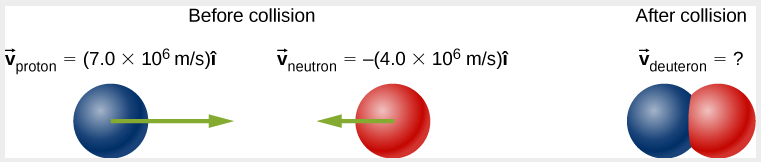
\includegraphics[width=0.5\textwidth]{deuteron.png}
\caption{\label{fig:deu} A proton and neutron collide.}
\end{figure}

\end{document}
